
%%%%%%%%%%%%%%%%%%%%%%% file typeinst.tex %%%%%%%%%%%%%%%%%%%%%%%%%
%
% This is the LaTeX source for the instructions to authors using
% the LaTeX document class 'llncs.cls' for contributions to
% the Lecture Notes in Computer Sciences series.
% http://www.springer.com/lncs       Springer Heidelberg 2006/05/04
%
% It may be used as a template for your own input - copy it
% to a new file with a new name and use it as the basis
% for your article.
%
% NB: the document class 'llncs' has its own and detailed documentation, see
% ftp://ftp.springer.de/data/pubftp/pub/tex/latex/llncs/latex2e/llncsdoc.pdf
%
%%%%%%%%%%%%%%%%%%%%%%%%%%%%%%%%%%%%%%%%%%%%%%%%%%%%%%%%%%%%%%%%%%%


\documentclass[francais,runningheads,a4paper]{llncs}

\usepackage[frenchb]{babel}
\usepackage{caption}
\usepackage[T1]{fontenc}
\usepackage{lmodern}

\usepackage{amssymb}
\setcounter{tocdepth}{3}
\usepackage{graphicx}

\usepackage{url}
\urldef{\mailsa}\path|dylan.baptiste@etudiant.univ-reims.fr|
\urldef{\mailsb}\path|stephane.cormier@univ-reims.fr|    
\urldef{\mailsc}\path|shufan.jiang@univ-reims.fr|
\newcommand{\keywords}[1]{\par\addvspace\baselineskip
\noindent\keywordname\enspace\ignorespaces#1}

\begin{document}
\mainmatter  % start of an individual contribution

% first the title is needed
\title{Évaluation des apports d'un reseau de neurones antagoniste pour une classification semi-supervisé de textes français issue d'une base de données faiblement labellisés}

% a short form should be given in case it is too long for the running head
\titlerunning{Apports d'un GAN pour une classification semi-supervisé}

% the name(s) of the author(s) follow(s) next
%
% NB: Chinese authors should write their first names(s) in front of
% their surnames. This ensures that the names appear correctly in
% the running heads and the author index.
%
\author{Dylan Baptiste \and Stéphane Cormier \and Shufan Jiang}
%
\authorrunning{Apports d'un GAN dans une classification semi-supervisé}
% (feature abused for this document to repeat the title also on left hand pages)

% the affiliations are given next; don't give your e-mail address
% unless you accept that it will be published
\institute{Université de Reims Champagne-Ardenne\\
\mailsa\\
\mailsb\\
\mailsc\\}

%
% NB: a more complex sample for affiliations and the mapping to the
% corresponding authors can be found in the file "llncs.dem"
% (search for the string "\mainmatter" where a contribution starts).
% "llncs.dem" accompanies the document class "llncs.cls".
%

\toctitle{}
\tocauthor{}
\maketitle

\graphicspath{ {../src/} }

\begin{abstract}
Les tâches de classifications de textes se heurtent souvent au problème de bases de données peu voir pas labellisé. Ici nous nous intéressons au apports de l'ajout d'un GAN afin d'artificiellement créer des données labellisés. Le but est d'améliorer les performances d'un classifieur qui ne se serait entraîné que sur des données labellisé issue d'une petite base de données.
\keywords{réseau de neurones, réseaux antagonistes génératifs, traitement du language, classification, semi-supervisé}
\end{abstract}

\tableofcontents

\listoffigures

\listoftables

\section{Contexte}
Ce travail à été réalisé dans le cadre d'un TER (Travail d'Étude et de Recherche) par Dylan Baptiste, étudiant en 2\ieme{} année de Master, supervisé par Shufan Jiang, doctorante, et Stéphane Cormier, enseignant-chercheur, à l'Université de Reims Champagne-Ardenne.

presentation des données\dots

\section{État de l'art}

	\subsection{Bidirectional Encoder Representations from Transformers}
	en fr "Représentations d'encodeur bidirectionnel à partir de transformateurs"
	BERT, CamemBERT\dots
	explications des ouputs de tels modeles
	
	\subsection{Réseaux antagonistes génératifs}
	GAN, Conditional GAN\dots
	
\section{Architecture}
	
	\subsection{Générateur}
	
	\subsection{Discriminateur}

	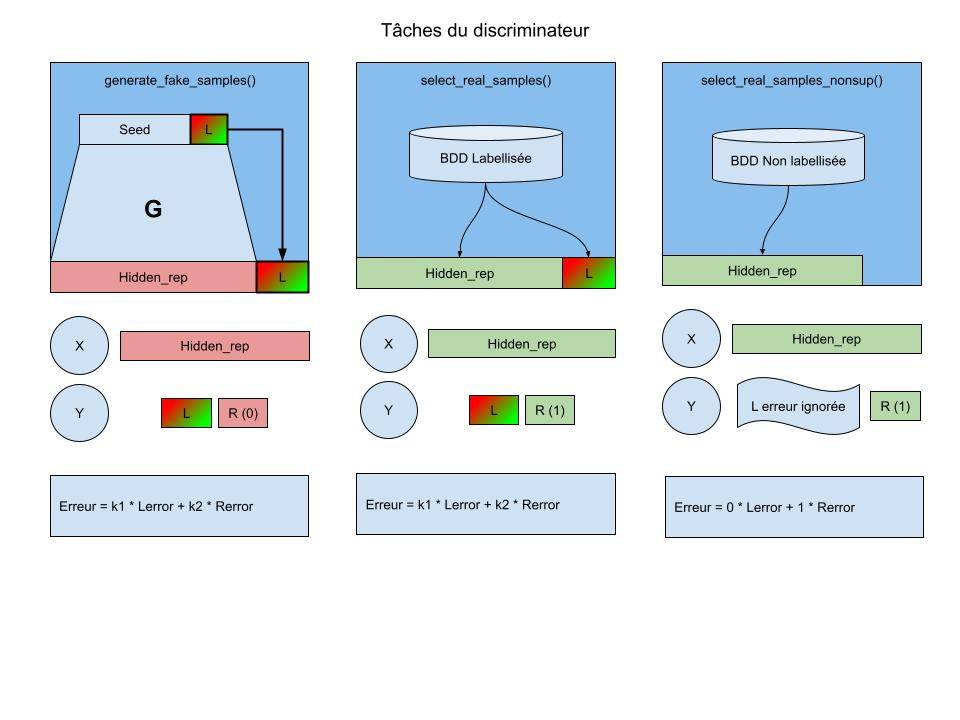
\includegraphics[width=\textwidth]{tacheD.jpg}

	\subsection{GAN}

	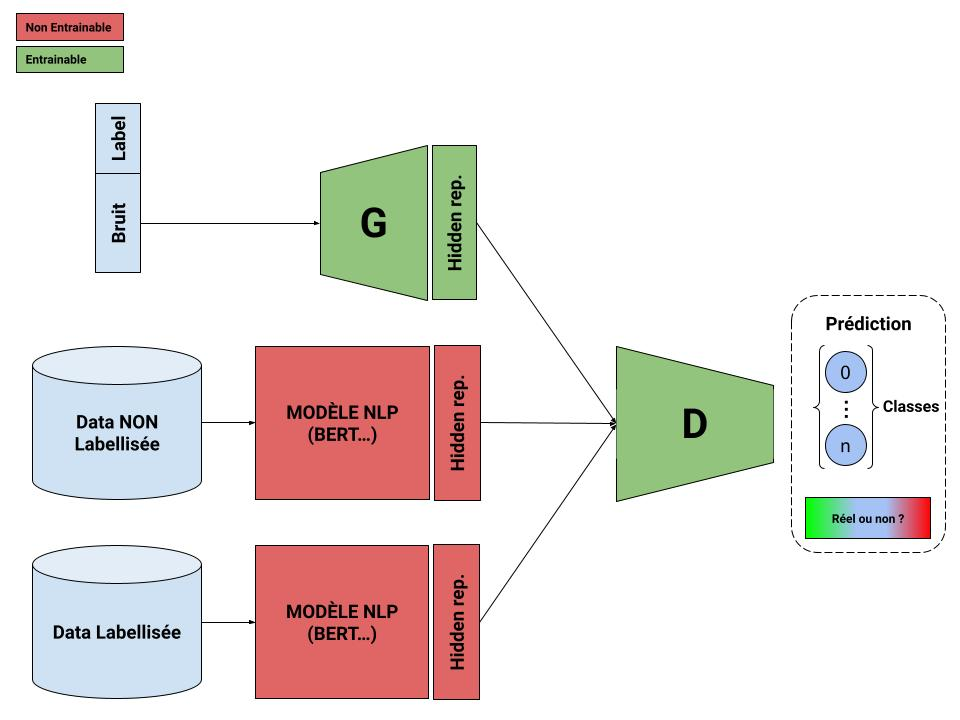
\includegraphics[width=\textwidth]{Architectutre_Entrainement.jpg}

	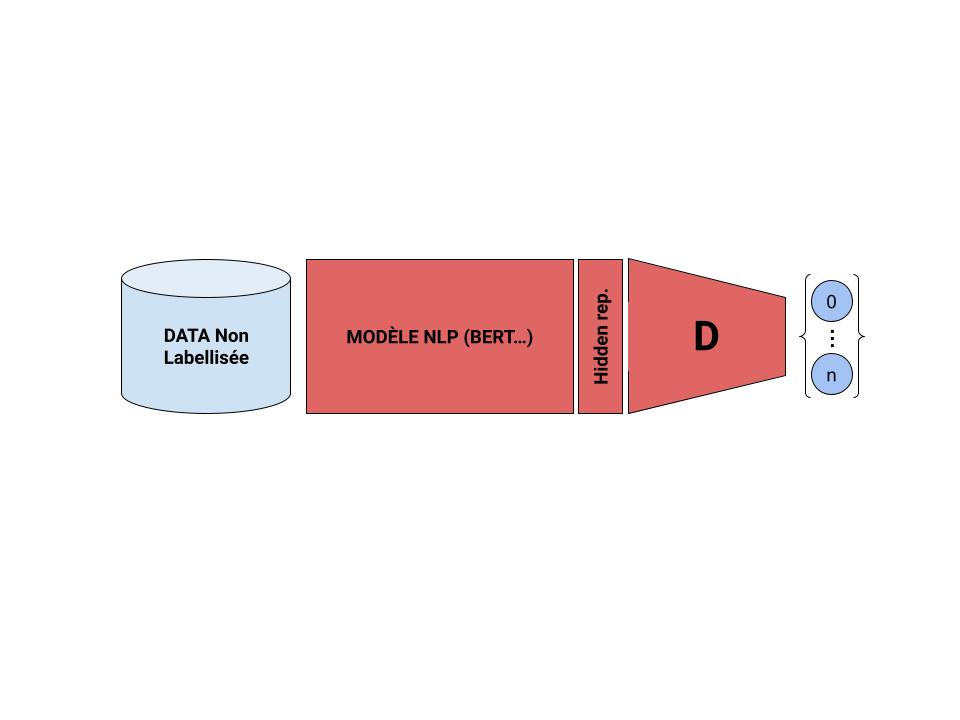
\includegraphics[width=\textwidth]{Architecture_Utilisation.jpg}
	
\section{Entraînement}

	- somme de 2 bce (label, réalité)

	\subsection{Supervisé}

	\subsection{Semi-supervisé}
		\subsubsection{Competion ou coopération ?}
		\subsubsection{Stabilisation du Générateur et Discriminateur}
\section{Evaluation}
\subsection{Mesures utilisées}
recall, precision, f1 score , APS,AUC
au sein d'une cross validation (5folds, équilibre pour l'entraînement)

\subsection{Comparaison des mesures}
	
\section{Conclusion et perspectives}
perspectives:
generation au niveau des token, utilisation d'un modèle NLP entraîné sur le corpus que l'on souhaite classer 
	

\end{document}
